\section{Summary of first half of lab work}
\begin{frame}
    \frametitle{Summary of first half of lab work}
    \begin{itemize}
        \item Familiarization with Kilobots
        \item Establishing communication between two Kilobots (speaker and listener)
        \item Implementing naive algorithm for orbiting of Kilobots (star and planet)
        \item Moving towards the direction of light source
        \item Synchronizing phase of blinking LEDs
    \end{itemize}
\end{frame}

\begin{frame}
\frametitle{Flowchart}
\begin{figure}[H]
	\centering
	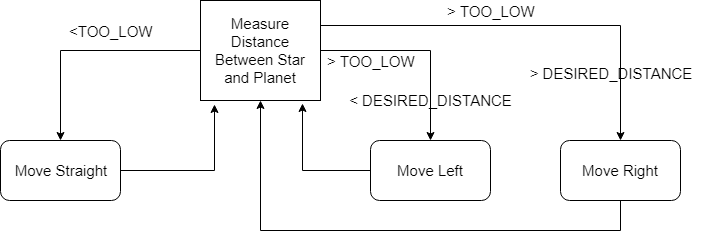
\includegraphics[scale=0.24]{orbiting}
\end{figure}
\end{frame}

\begin{frame}
\frametitle{Naive orbiting algorithm}
\framesubtitle{Demonstration}
\begin{figure}[H]
	\begin{center}
		\fbox{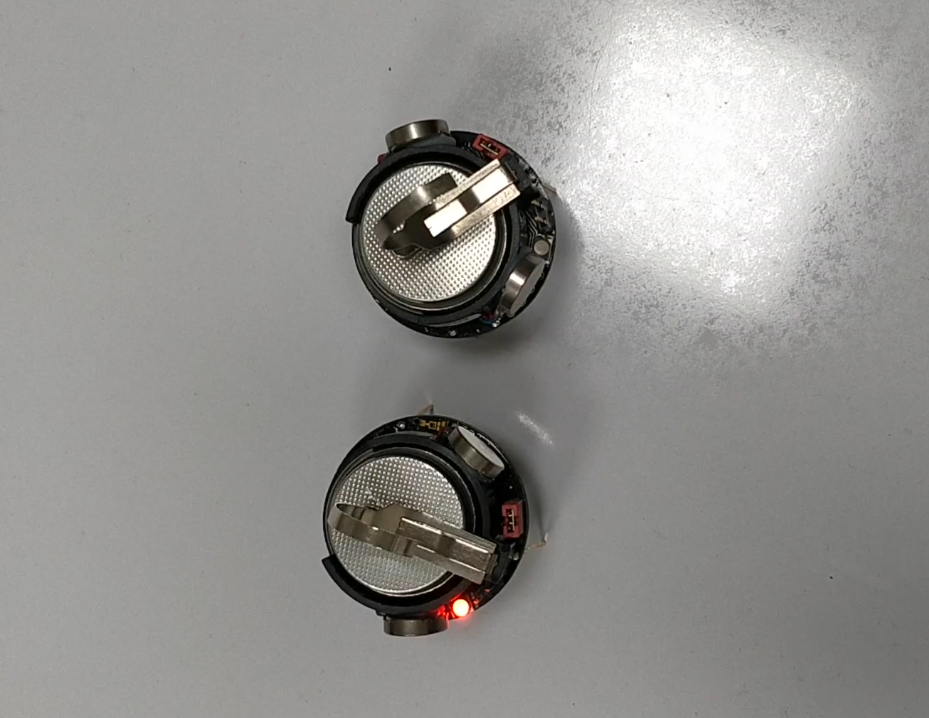
\includegraphics[width=2in]{orbit}}\\
		\vspace{0.2cm}
		\caption{\href{https://youtu.be/jPBkttH8Q2o}{Naive orbiting algorithm}}
	\end{center}
\end{figure}
\end{frame}